	From \eqref{eq:11/10/4/22},
the reflection of $\vec{Q}$ is 
\begin{align}
\vec{R}  
= \myvec{5\\-3}
\end{align}
Letting
\begin{align}
\vec{A} = \myvec{x\\0},
\end{align}
since 
$\vec{P},
\vec{A},  
\vec{R}  
$
are collinear, 
		from \eqref{prop:lin-dep-rank},
\begin{align}
	\myvec{
		1 & 1 & 2 
		\\ 
		1 & 5 & -3 
		\\
		1 & x & 0 }
	\xleftrightarrow[R_3=R_3 - R_1]{R_2 = R_2 - R_1}
	\myvec{
		1 & 1 & 2 
		\\ 
		0 & 4 & -5 
		\\
		0 & x-1 & -2 }
	\\
	\xleftrightarrow[]{R_3 = 4R_3 - \brak{x-1}R_2}
	\myvec{
		1 & 1 & 2 
		\\ 
		0 & 4 & -5 
		\\
		0 & 0 & 5x-13 }
	\implies x = \frac{13}{5}
\end{align}
See  
\figref{fig:chapters/11/10/4/22/1}.
\begin{figure}[H]
\centering
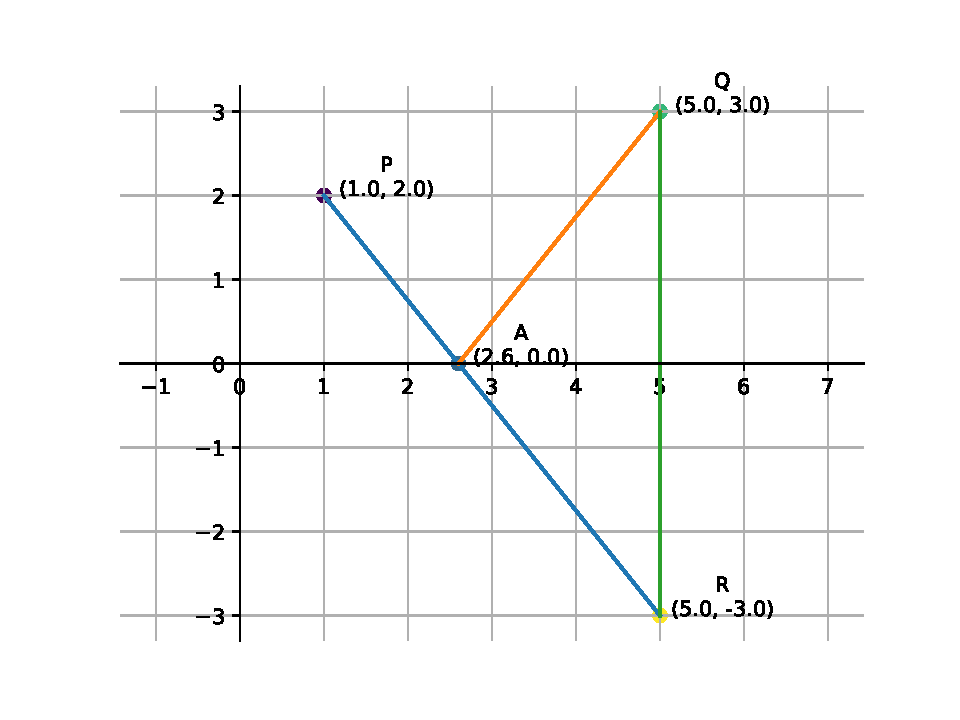
\includegraphics[width=0.75\columnwidth]{chapters/11/10/4/22/figs/fig.pdf}
\caption{}
\label{fig:chapters/11/10/4/22/1}
\end{figure}



